% Problem 4.4: Monte Carlo integration (II)
% Notes and checklist: ../Exercises/4.04-mc-integration-2-metropolis/README.md
% Figures:            \includegraphics{4.04-mc-integration-2-metropolis/figures/<name>}
\exercise{4}{Monte Carlo integration (II)}

The integral $\mathcal I$ of problem~4.3 is now computed with points from a Markov chain whose
stationary distribution is $w(\mathbf r) = (2\pi)^{-3/2}e^{-r^2/2}$, built with the Metropolis
algorithm \cite{Carlon2025}. One step from the current point $\mathbf r$:
\begin{enumerate}
  \item propose $\mathbf r' = \mathbf r + \boldsymbol\delta$, with the three components of
        $\boldsymbol\delta$ independent and uniform in $[-h/2, h/2]$;
  \item accept with probability $A = \min\big(1, e^{-(r'^2-r^2)/2}\big)$, otherwise keep $\mathbf r$.
        A rejected move still counts: the old point is added to the sample again.
\end{enumerate}
The proposal is symmetric, $g(\mathbf r\to\mathbf r') = g(\mathbf r'\to\mathbf r)$, so
$P(\mathbf r\to\mathbf r')/P(\mathbf r'\to\mathbf r) = A(\mathbf r\to\mathbf r')/A(\mathbf r'\to\mathbf r)
= w(\mathbf r')/w(\mathbf r)$, which is detailed balance. Every point can be reached in a finite
number of steps for any $h > 0$, so the chain is ergodic and $w$ is its unique stationary
distribution. Only the ratio $w(\mathbf r')/w(\mathbf r)$ enters, so the normalisation of $w$ is not
needed. All runs use seed~1 with one generator used in order through the notebook.

\subsection{Trajectories and equilibrium distribution}

Figure~\ref{fig:4.4-traj} shows the $(x,y)$ projection of chains of $10^4$ steps. With $h = 1$
(acceptance 0.81) the chain from the origin fills the Gaussian blob $|x|,|y| \lesssim 3$, and the chain
from $(10,10,10)$ walks to the origin in a few hundred steps and then stays there. With $h = 0.1$
(acceptance 0.94--0.99) the chain performs a slow random walk: from the origin it explores only a part
of the blob, and from $(10,10,10)$ it only just reaches the centre at the end of the run.

\begin{figure}[htbp]
  \centering
  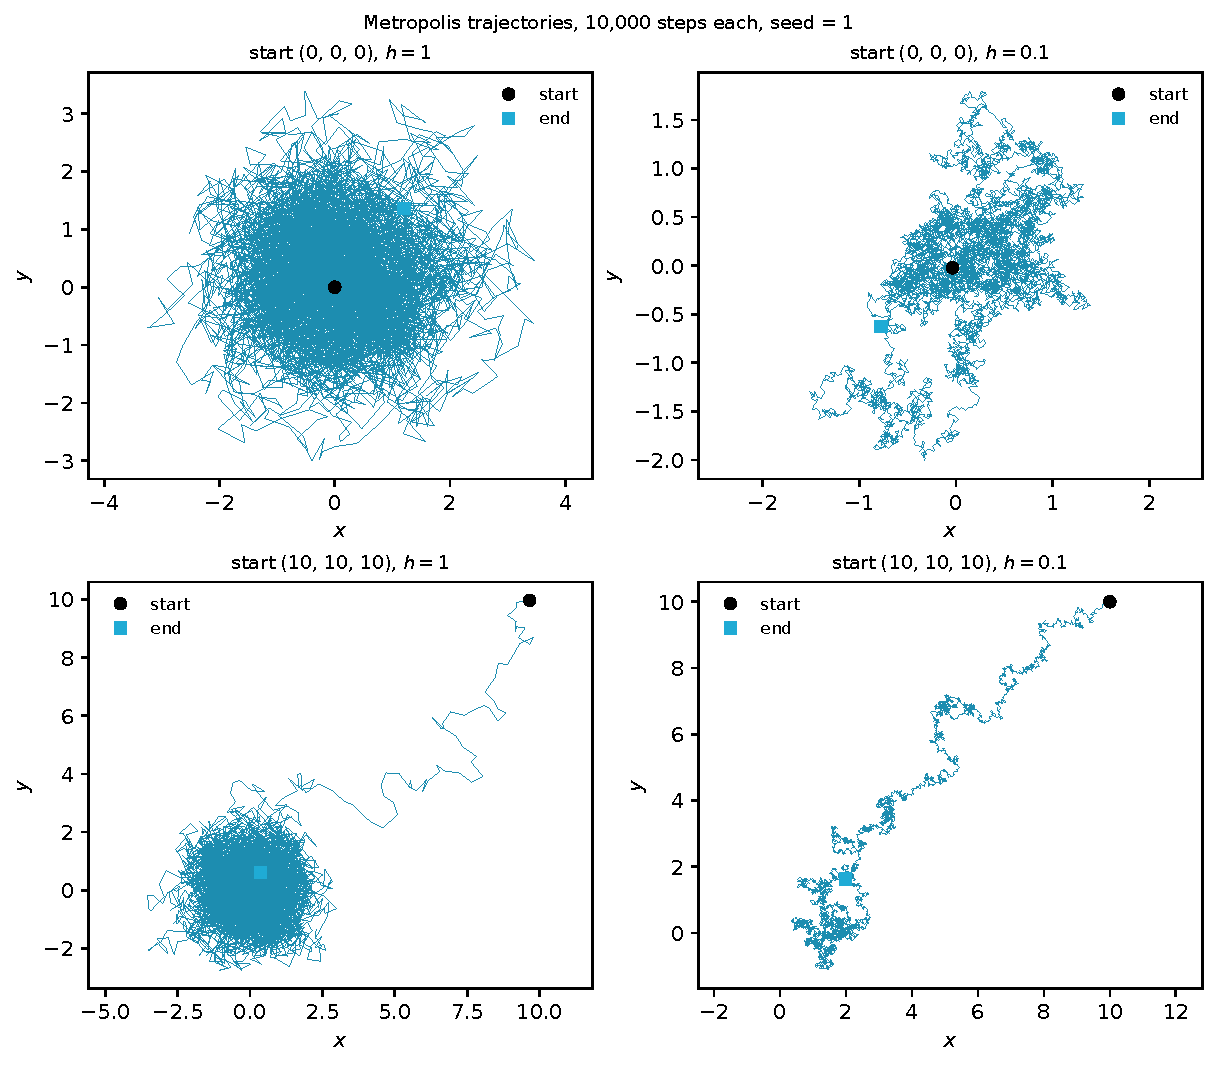
\includegraphics[width=0.72\linewidth]{4.04-mc-integration-2-metropolis/figures/trajectories}
  \caption{$(x,y)$ projection of Metropolis chains of $10^4$ steps, starting at $(0,0,0)$ (top) and
    $(10,10,10)$ (bottom), with step size $h = 1$ (left) and $h = 0.1$ (right). Acceptance rates 0.81,
    0.99, 0.81 and 0.94. Seed 1.}
  \label{fig:4.4-traj}
\end{figure}

To check the stationary distribution we run $10^6$ steps from the origin, after discarding $2\times10^4$
equilibration steps (well above the $N_{\text{eq}}$ found in the third subsection). The histograms in
figure~\ref{fig:4.4-hist} follow the exact marginals, $e^{-x^2/2}/\sqrt{2\pi}$ for each coordinate and
the Maxwell density $\sqrt{2/\pi}\,r^2e^{-r^2/2}$ for $r = |\mathbf r|$. For $h = 1$ the second moments
are $\avg{x^2}, \avg{y^2}, \avg{z^2} = 1.002, 1.000, 1.001$ (exact 1). For $h = 0.1$ they are $1.023,
0.964, 1.025$ and the histograms are visibly noisier: the same number of points, but far fewer
independent ones.

\begin{figure}[htbp]
  \centering
  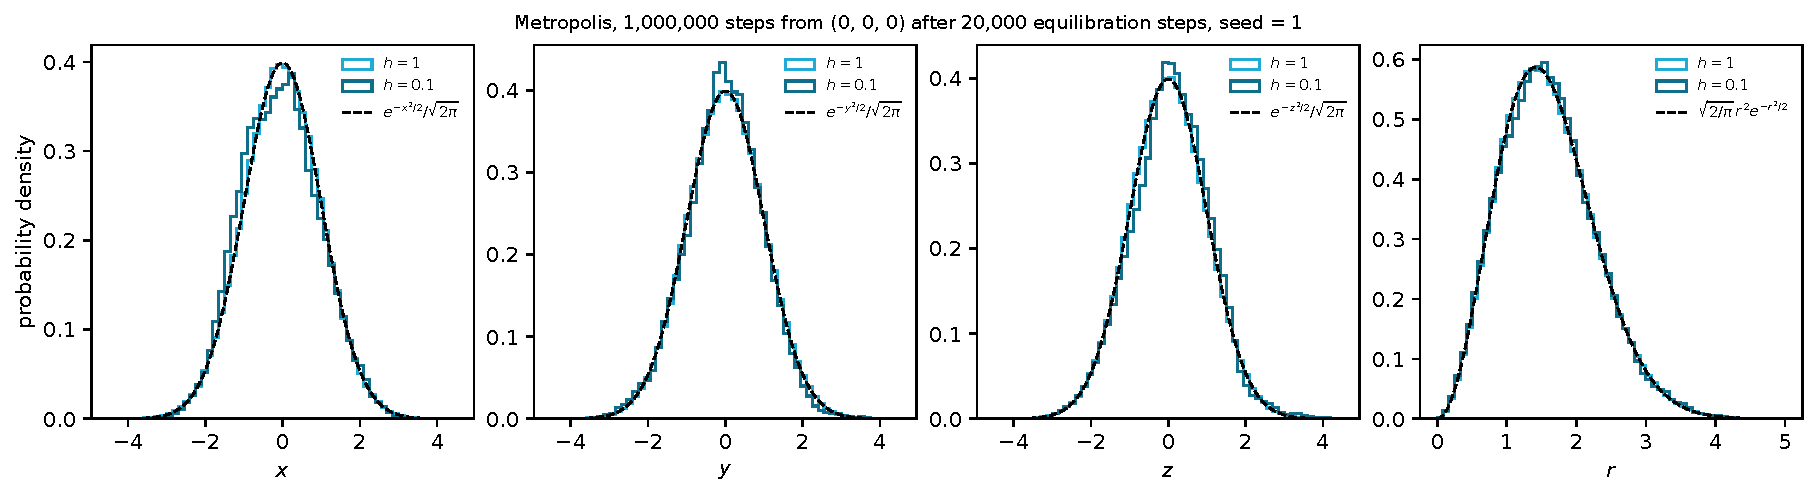
\includegraphics[width=\linewidth]{4.04-mc-integration-2-metropolis/figures/histograms}
  \caption{Histograms (60 bins) of $x$, $y$, $z$ and $r$ from Metropolis chains of $10^6$ steps
    started at the origin, after $2\times10^4$ discarded equilibration steps, for $h = 1$ and
    $h = 0.1$. Dashed: exact densities. Seed 1.}
  \label{fig:4.4-hist}
\end{figure}

\subsection{Estimate of the integral}

As in problem~4.3, $\mathcal I = (2\pi)^{3/2}\avg{f}_w$ with $f = (x+y+z)^2$, but the average now runs
over the points of the chain. Successive points are correlated, so the naive error $s_f/\sqrt N$ is too
small. We use blocking: the chain is cut into blocks of $B$ steps, and the spread of the block means
gives the error. When $B$ is much longer than the correlation time the block means are independent,
and the error stops growing with $B$ (figure~\ref{fig:4.4-blocking}). The error at $B = 8192$ defines
the integrated autocorrelation time through
$\sigma_{\text{block}}^2 = 2\tau_{\text{int}}\,s_f^2/N$.

\begin{table}[htbp]
  \centering
  \caption{Estimates of $\mathcal I$ with $N = 10^6$ points. Metropolis: chains from the origin after
    $2\times10^4$ discarded steps, error from blocking with $B = 8192$. Seed 1.}
  \label{tab:4.4-integral}
  \begin{tabular}{lcccc}
    \toprule
    method & $\mathcal I$ & naive error & $\tau_{\text{int}}$ (steps) & deviation \\
    \midrule
    exact                       & $47.249$           & --    & --          & -- \\
    Gaussian sampling (4.3)     & $47.241 \pm 0.067$ & 0.067 & $1/2$       & $-0.1\sigma$ \\
    Metropolis, $h = 1$         & $47.64 \pm 0.42$   & 0.067 & $19 \pm 2$   & $+0.9\sigma$ \\
    Metropolis, $h = 0.1$       & $43.5 \pm 2.3$     & 0.059 & $770 \pm 100$ & $-1.6\sigma$ \\
    \bottomrule
  \end{tabular}
\end{table}

\kulbox[5pt]{Metropolis with $N = 10^6$ steps gives $\mathcal I = 47.64 \pm 0.42$ ($h = 1$) and
$43.5 \pm 2.3$ ($h = 0.1$), both compatible with the exact $47.249$. The error is $\sqrt{2\tau_{\text{int}}}$
times that of direct Gaussian sampling: 6 times larger for $h = 1$ and 40 times for $h = 0.1$.}

The naive errors in table~\ref{tab:4.4-integral} are about the same as for Gaussian sampling, because
the points have the right distribution. They ignore the correlations and are therefore wrong. For
$h = 0.1$ the blocking curve has not fully levelled off at $B = 8192$ (the chain contains only about
$N/2\tau_{\text{int}} \approx 600$ independent points), so that error bar is a slight underestimate.

\begin{figure}[htbp]
  \centering
  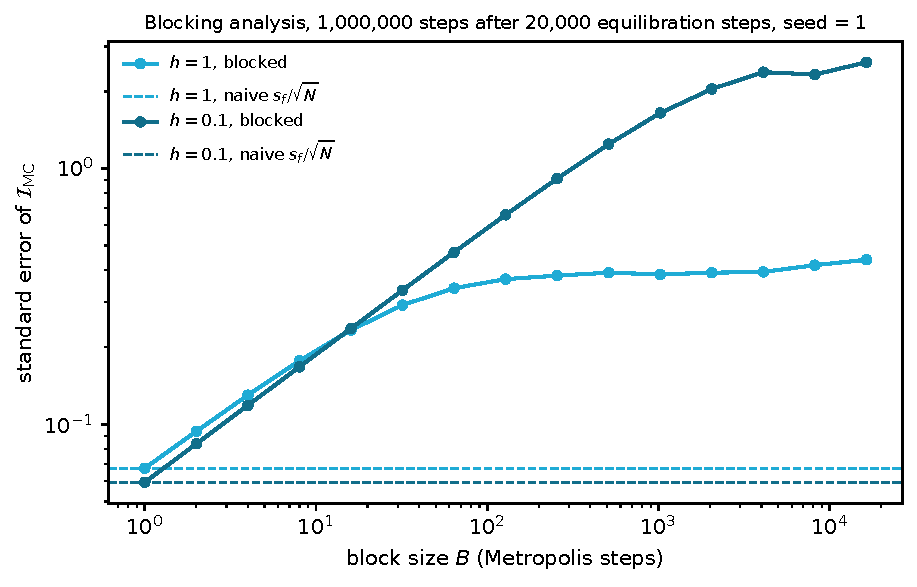
\includegraphics[width=0.72\linewidth]{4.04-mc-integration-2-metropolis/figures/blocking}
  \caption{Blocking analysis: standard error of $\mathcal I_{\text{MC}}$ against block size $B$ for the
    $10^6$-step chains of figure~\ref{fig:4.4-hist}. Dashed: the naive error $s_f/\sqrt N$ ($B = 1$).
    Seed 1.}
  \label{fig:4.4-blocking}
\end{figure}

\subsection{Equilibration time}

Starting from $(10,10,10)$, $r^2 = 300$ has to relax to its equilibrium mean $\avg{r^2} = 3$. One chain is
noisy, so we average $r^2(t)$ over 100 independent chains of $2\times10^4$ steps. In equilibrium
$r^2 \sim \chi^2_3$ has variance 6, so the chain average fluctuates by $\sqrt{6/100} = 0.24$. We define
$N_{\text{eq}}$ as the first step at which the average drops below $3 + 2\sqrt{6/100} = 3.49$
(figure~\ref{fig:4.4-eq}).

For small $h$ the relaxation can be estimated. A uniform step has variance $h^2/12$ per component, and to
first order Metropolis gives a mean displacement $\frac{h^2}{24}\nabla\ln w = -\frac{h^2}{24}\mathbf r$
per step. Then $\avg{r^2} - 3 \approx 297\,e^{-h^2t/12}$, so
\begin{equation}
  N_{\text{eq}} \approx \frac{12}{h^2}\ln\frac{297}{0.49} \propto \frac{1}{h^2} .
\end{equation}

\begin{table}[htbp]
  \centering
  \caption{Equilibration time from $(10,10,10)$, 100 chains of $2\times10^4$ steps, seed 1.}
  \label{tab:4.4-neq}
  \begin{tabular}{ccc}
    \toprule
    $h$ & measured $N_{\text{eq}}$ & small-$h$ estimate \\
    \midrule
    1   & 205  & 77   \\
    0.1 & 8485 & 7689 \\
    \bottomrule
  \end{tabular}
\end{table}

The estimate works for $h = 0.1$ (table~\ref{tab:4.4-neq}). For $h = 1$ it is too optimistic: far from
the origin $r'^2 - r^2 \approx 2\,\mathbf r\cdot\boldsymbol\delta$ is large, so nearly every outward step
is rejected and nearly every inward step accepted. The chain then moves inward at a roughly constant
speed of about 0.1 per step ($r$ goes from 17.3 to about 3 in some 150 steps) instead of relaxing
exponentially. The $2\times10^4$ discarded steps in the other subsections are well above both values.

\begin{figure}[htbp]
  \centering
  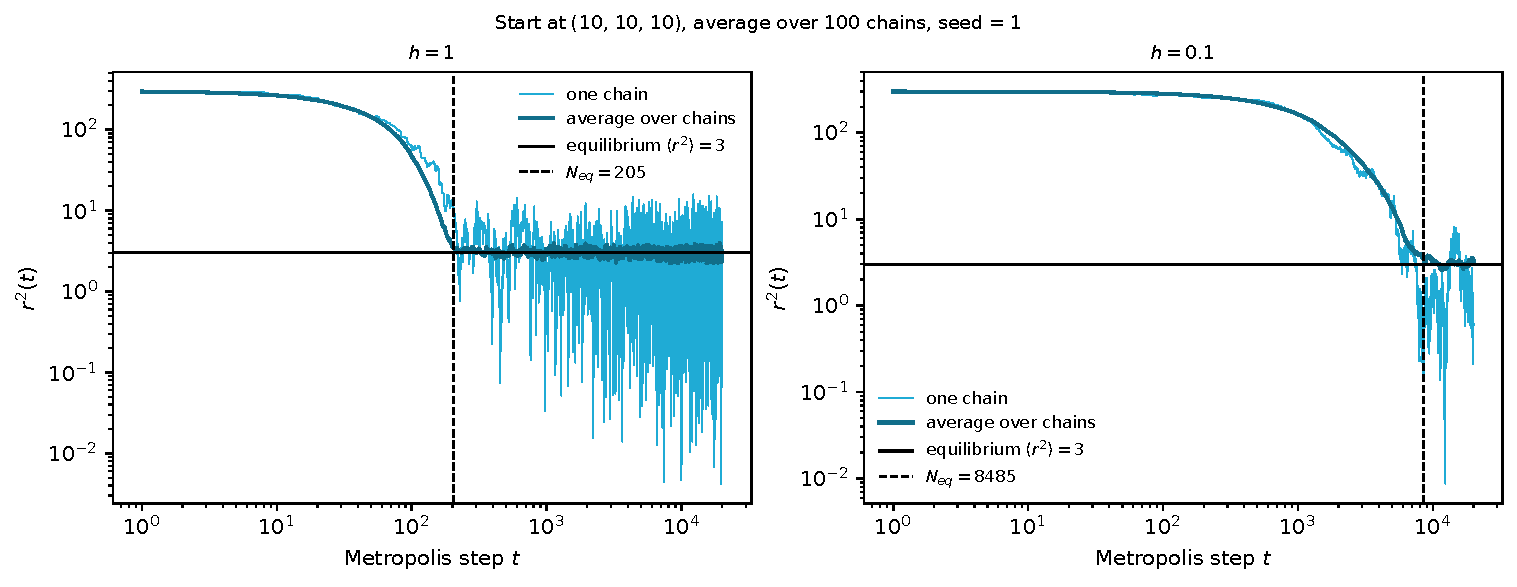
\includegraphics[width=\linewidth]{4.04-mc-integration-2-metropolis/figures/equilibration}
  \caption{Relaxation of $r^2(t)$ from $(10,10,10)$ for $h = 1$ (left) and $h = 0.1$ (right): one chain
    and the average over 100 chains of $2\times10^4$ steps. Dashed: $N_{\text{eq}}$, where the average
    first drops below $3.49$. Seed 1.}
  \label{fig:4.4-eq}
\end{figure}

\subsection{Gaussian sampling or Metropolis?}

The step size $h$ controls a trade-off (figure~\ref{fig:4.4-hscan}). For small $h$ almost every proposal
is accepted, but the steps are tiny and the chain diffuses, with $\tau_{\text{int}} \propto 1/h^2$. For
large $h$ the proposals land far in the tails and are rejected, so the chain stands still. The optimum
lies in between, $h \approx 2$--$5$ with acceptance 0.25--0.6, where $\tau_{\text{int}} \approx 5$ steps.

\begin{table}[htbp]
  \centering
  \caption{Acceptance rate and $\tau_{\text{int}}$ of $f = (x+y+z)^2$ against $h$, from $5\times10^5$
    steps per $h$ after $2\times10^4$ discarded steps, blocks of 8192 steps. Seed 1.}
  \label{tab:4.4-hscan}
  \begin{tabular}{lccccccccc}
    \toprule
    $h$ & 0.1 & 0.2 & 0.5 & 1 & 2 & 3 & 5 & 10 & 20 \\
    \midrule
    acceptance           & 0.98 & 0.96 & 0.90 & 0.81 & 0.63 & 0.48 & 0.26 & 0.053 & 0.006 \\
    $\tau_{\text{int}}$  & 1041 & 317  & 69   & 18.5 & 5.5  & 5.1  & 4.6  & 15    & 147 \\
    \bottomrule
  \end{tabular}
\end{table}

For this integral direct Gaussian sampling is clearly better. Even at the best $h$, a chain of $N$ steps
is worth only $N/(2\tau_{\text{int}}) \approx N/10$ independent points, while one Metropolis step costs
about as much as drawing three Gaussian numbers (four uniform numbers and an exponential). Gaussian
sampling is therefore at least ten times cheaper for the same error, and it needs no equilibration and no
blocking analysis. Metropolis becomes the method of choice when $w$ cannot be sampled directly, for
instance for many coupled variables as in the Ising model, or when its normalisation is unknown.

\begin{figure}[htbp]
  \centering
  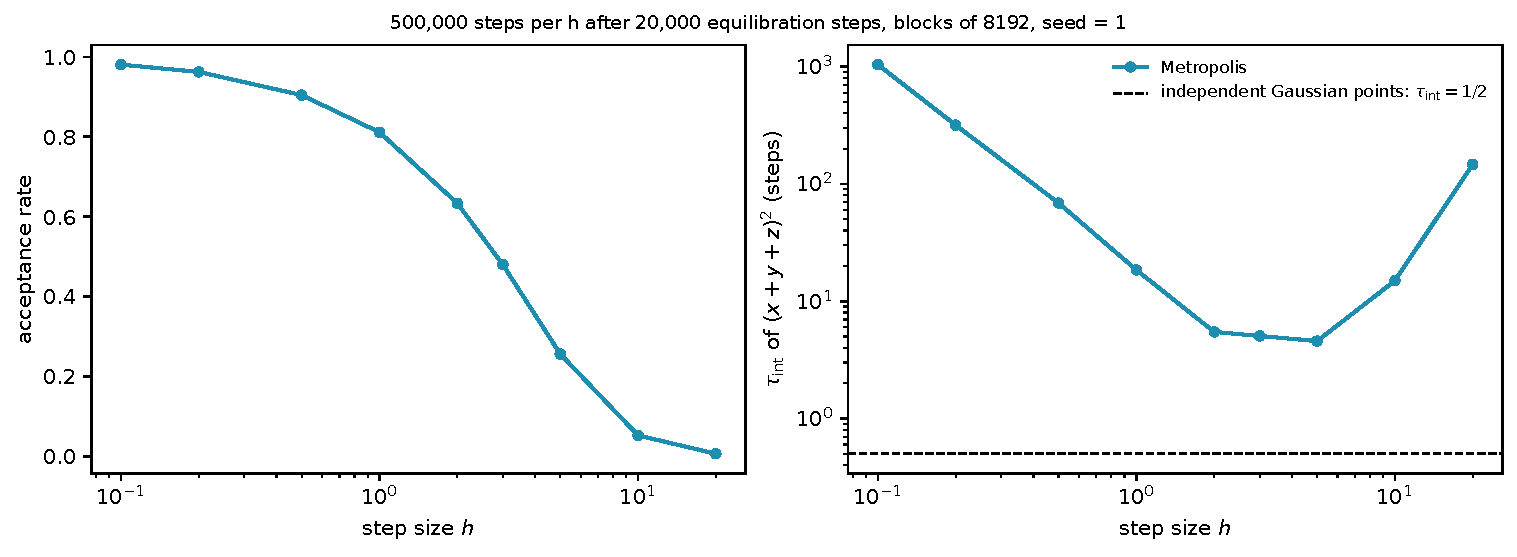
\includegraphics[width=0.85\linewidth]{4.04-mc-integration-2-metropolis/figures/h_scan}
  \caption{Step-size scan: acceptance rate (left) and integrated autocorrelation time of
    $(x+y+z)^2$ (right) against $h$, $5\times10^5$ steps per $h$ after $2\times10^4$ discarded steps,
    blocks of 8192 steps. Dashed: $\tau_{\text{int}} = 1/2$ for independent Gaussian points. Seed 1.}
  \label{fig:4.4-hscan}
\end{figure}
